\section{Impedance from a mutual inductance}

In our lab we frequently use mutual inductances to couple circuit elements.
It is very useful to derive a formula for the impedance looking into a circuit fragment with an inductive coupling.
Consider the circuit shown in Figure \ref{Fig:mutualInductance}.
The flux in $L_1$ is
\begin{equation}
\Phi_1 = I_1 L_1 - M I_2
\end{equation}
and the flux in $L_2$ is
\begin{equation}
\Phi_2 = I_2 L_2 - M I_1 \, .
\end{equation}
The voltage in the coupled loop is
\begin{equation}
V_2 = - I_2 Z \, .
\end{equation}
Differentiating the flux in the loop gives
\begin{align}
\dot{\Phi}_2 &= V_2 \\
\dot{I}_2 L_2 - \dot{I}_1 M &= - I_2 Z \,.
\end{align}
We now represent all amplitudes as phasors, which turns the previous equation into
\begin{align}
i \omega I_2 L_2 - i \omega I_1 M &= - I_2 Z \\
I_2 &= \frac{i \omega M I_1}{i\omega L_2 + Z} \, .
\end{align}
Differentiating the flux in $L_1$ gives
\begin{align}
V_1 &= \dot{\Phi}_1 \\
&= i \omega I_1 L_1 - \frac{(i \omega)^2 M^2 I_1}{i \omega L_2 + Z} \\
Z_{\text{in}} \equiv V_1/I_1 &= i \omega L_1 + \frac{(\omega M)^2}{i \omega L_2 + Z} \, .
\end{align}
The first term is the expected contribution from $L_{1}$ while the second term is the effect of the loop.

\begin{figure}
\begin{centering}
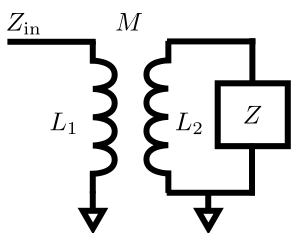
\includegraphics[width=7cm]{mutualInductance.pdf} 
\par\end{centering}
\caption{Circuit fragments coupled through a mutual inductance $M$}
\label{Fig:mutualInductance}
\end{figure}
